\documentclass[SE,authoryear,toc]{lsstdoc}

% lsstdoc documentation: https://lsst-texmf.lsst.io/lsstdoc.html
\input{meta}

% Package imports go here.
\usepackage{graphicx}

% Local commands go here.
\graphicspath{{figures/}} %Setting the graphicspath

%If you want glossaries
%\input{aglossary.tex}
%\makeglossaries

\title{Project-wide Documentation Proposal for Rubin Observatory Operations}

% Optional subtitle
\setDocSubtitle{(Report from the Rubin Observatory Documentation Working Group)}

\author{%
Matthew Rumore,
Chuck Claver,
David Cabrera,
Rob McKercher,
John Andrew,
Diane Hascall,
Patrick Ingraham,
Tony Johnson,
Kristen Metzger,
Austin Roberts,
Jonathan Sick.
}

\setDocRef{SITCOMTN-014}
\setDocUpstreamLocation{\url{https://github.com/lsst-sitcom/sitcomtn-014}}

\date{\vcsDate}

% Optional: name of the document's curator
\setDocCurator{Matthew Rumore}

\setDocAbstract{%
This technical note is a report to recommend a future state for Rubin Observatory Operations documentation by the Project-wide Documentation Working Group.
This proposal presents a high-level documentation strategy for Rubin Observatory Operations with suggested methodologies to transition Construction Project documents and organizations for the technical documentation package needed to establish construction completeness and operational readiness.
It responds to charge items 3 in the \textit{Charge to the Documentation Working Group}, \citeds{LSE-489}.
Migration plans, schedule and resources to migrate to the future state for this documentation will be reported in another techincal report, \citeds{RTN-076}.  Implementation of this proposal (or its equivelent) is a key deliverable from the Rubin Observatory Construction Project to Operations.
}

% Change history defined here.
% Order: oldest first.
% Fields: VERSION, DATE, DESCRIPTION, OWNER NAME.
% See LPM-51 for version number policy.
\setDocChangeRecord{%
  \addtohist{0.0}{2021-06-26}{First draft of preliminary content.}{Chuck Claver}
  \addtohist{0.1}{2021-08-30}{Input to Documentation Portal.}{Jonathan Sick}
  \addtohist{0.2}{2021-09-14}{Preliminary content, Portal architecture and effort.}{Chuck Claver, Jonathan Sick}
  \addtohist{0.3}{2022-11-18}{Incorporate draft from Confluence pages and shared files as pre-draft.}{David Cabrera, Matthew Rumore}
  \addtohist{0.4}{2024-03-20}{Finalize roadmap; transfer implementation content to RTN-076.}{Matthew Rumore, Leanne Guy}
  \addtohist{1.0}{2024-04-09}{Finalize roadmap; transfer implementation content to RTN-076.}{Matthew Rumore, Leanne Guy}
  \addtohist{1.1}{2024-04-25}{Edits.}{Chuck Claver}
  \addtohist{1.2}{2024-04-26}{Placeholder modification for version control.}{Authors TBD}
}

\graphicspath{{./}{figures/}}
\setcounter{tocdepth}{2}


\begin{document}

% Create the title page.
\maketitle
% Frequently for a technote we do not want a title page  uncomment this to remove the title page and changelog.
% use \mkshorttitle to remove the extra pages

% ADD CONTENT HERE
% You can also use the \input command to include several content files.

\section{Introduction}

Put basic description of approach and report structure here.

This report include details on the following topics:

\begin{itemize}

\item DocumentationViews
	\begin{itemize}
	\item ProductView
	\item AccessView
	\item  StorageView
	\item TopicView
	\end{itemize}
	
\item Implementation Plan
	\begin{itemize}
	\item PrimarySources
	\item DocumentationPortal
	\item DocuSharePath
	\item PDMWorksPath
	\item Resources \& Responsibilities
	\item Schedule
	\item TransitionPlan
	\end{itemize}
	
\item RiskAssessment

\end{itemize}


\section{Documentation Views}
\label{sec:views}

There are four \emph{Documentation Views} with a set of customized categories and subcategories developed by the Documentation Working Group to functionally describe and organize the technical documentation for the Rubin Observatory.
The views and categories will assist those responsible for technical documentation when considering the informational needs and interests of users, communities, operations staff, and other stakeholders.
Each view is represented by a \emph{tree structure}, a widely used way of representing hierarchical structures typically in a graphical form.
Examples in this proposal include classical node-link diagrams and tree view outlines that are built with \emph{branches} of connected nodes, or \emph{leaf-nodes}, starting from \emph{root-nodes} representing the highest level in the hierarchy.
Different tree structure diagrams can be used depending on the particular use case and how to effectively represent the information.
\citep{wiki-tree-diagram-cite}

Each View has its own purpose and they are designed to provide a framework structure to search, reference and retrieve currently available information consistently project-wide.
In addition, the Views will provide an orderly way to introduce new documentation and meet an extended goal of facilitate referencing and minimize replication.

The four views are:

\begin{itemize}

  \item \textbf{Product View} --- For organizing the ownership of documentation, describing internal systems and providing structure for linking and cross referencing documentation or informational dependencies.
  Notably includes the separation of Rubin Observatory Departments.

  \item \textbf{Storage View} --- For describing all project documentation storage locations and repositories.
  In conjunction with the Product View, identifying or determining the normative source of information.

  \item \textbf{Access View} --- For describing the user base and documentation applicable to their use cases.

  \item \textbf{Topic View} --- For searching and discovering documentation.

\end{itemize}

The owner or a designated responsible group will use the Documentation Views to develop an effective way to communicate the various pieces of documentation, how they are interconnected, dependencies or connections to another group's documentation, and utilization for various documents.
Stakeholders (e.g., internal and external technical groups, Rubin observatory communities) should be able to retrieve current information with consistency and reliability.
It is the responsibility of the owner or designated responsible group to keep this information up-to-date, organized, and readily available for stakeholders.
Stakeholders should provide regularly feedback over the course of operations.

This framework will improve the ability of pre-operations and operations staff to clearly establish and review information for construction completeness and operational readiness.
For example, all identified normative sources of information should be completed; or, a use case where multiple documents referencing one normative source more effectively serves multiple stakeholders than all related information in a single document.
The framework also supports managers and auditors in understanding a relevant system.
For example, a document that is referenced isn't identified as a normative source of information; a normative source of information is not located in an appropriate repository; or, identifying interfaces between systems to ensure operational requirements are met.

The following subsections propose how each Documentation View tree is constructed, various examples of use, recommendations for technical teams to consider, and capture any assessments of needed resources.

\subsection{Product View}

The \emph{Product View} is based on a common approach used in product management, a \emph{product tree diagram}.
The Documentation Working Group developed a framework customized for Rubin Observatory operations to facilitate the development of documentation and effective communication consistently project-wide.
The two primary purposes are to convey ownership and responsibility of technical documentation and more readily describe complicated systems with context and categorization.
The Product View allows one to identify specific documents as the normative source of information, then provide a manner which one can associate, link and cross reference documentation and informational dependencies from respective normative sources or references thereafter.
These goals support identifying and resolving gaps, miscommunications or error-likely situations.
The expected primary users are managers, product owners, engineers, specialists, technicians, and users which want to search downwards in a system's hierarchy.

The Product View will consist of product trees developed by the owning \emph{Rubin Observatory Departments}, their technical teams and product owners.
Each department's product tree(s) should be constructed to best organize and compartmentalize the set of \emph{products} that make up the complicated systems under their purview.
Products can span all manner of objects, such as department-specific categories, documents, hardware (systems, servers, networking, etc.), data (data sets, validation tests, verification artifacts, etc.), software interface information (alarms and notifications between hardware or software systems, support data storage and metadata schema, etc.), or subject-matter expert support.
Each department or group is responsible to manage the product trees in addition to updating technical documentation to support access to retrieve associated information, interfaces and requirements with consistency and reliability.
In light of this need, the Documentation Working Group recommends all Product View trees be available via one of the project repositories --- it is suggested to create an appropriate lsst.io website so departments and groups changes can easily make changes.

Products are defined by the owning department in terms of a system or set of systems which can be grouped or decomposed into subsystems or individual components that is appropriate for them and their stakeholders.
Referred to as the \emph{generic categories}, the customized categories for the Product View developed by the Documentation Working Group are predefined root-nodes and first set of leaf-nodes for a product tree.
The generic categories were developed to capture critical operational aspects of a product while being extendable to subsystems of a product, where the subsystem may be a product with subsystems in its own right; i.e., a \emph{Level-1 product} can be comprised of multiple Level-2 or lower-level subsystems, and those subsystems which are products are \emph{Level-2+ products}.
Note that these terms do not correspond to the construction phase definition of Work Breakdown Structure (WBS) or colloquial "subsystem" used across the construction project.
It is at the department's discretion on how to best organize and characterize these products and their product trees to manage their systems and flow of information; however, it is expected that all generic categories are associated with Level-1 and Level-2+ products either by construction or referenced information.
While there will be exceptions for low-level systems, the Product View and its generic categories are designed to robustly capture construction completeness and operations readiness because they should generate sufficient discussion between groups and stakeholders to ensure key information is identified and provided.

\subsubsection{Departments for Rubin Observatory operations}

The Rubin Observatory departments shall be described by their associated scope, systems and/or products descriptions, and contacts to identify managers, product owners, or other key personnel (e.g., organizational chart, contact list).
This section lists each department and respective scope.
Contact information should be available to individuals that require it, and it should be clear when it's appropriate to contact an individual or group (e.g., as a product owner).

\textbf{Director's Office} (DO) ---
The Vera C.\ Rubin Observatory Director's Office is responsible for the overall management of the observatory and the LSST survey, as well as fulfilling the mission of the observatory and realizing its vision.
The Director's Office includes a Directorate, Administrative Operations, Safety, Communications, and In-Kind Contributions teams.

\textbf{Observatory Operations} (OO) ---
The Chilean-based Rubin Observatory Operations Department is responsible for operating and maintaining the telescope, camera systems, and summit facilities in order to collect the raw imaging and housekeeping data needed by the LSST.
The primary tasks include maintaining the operating facilities, conducting the night-time survey operations, real-time assessment of image quality and observing efficiency, performing the daily calibration, and collecting and analyzing engineering data.

\textbf{Data Production} (DP) ---
The role of the Rubin Observatory Data Production department is to accept data from the Observatory's telescopes and ancillary systems; to process that data to generate science ready data products; to archive both raw data and derived data products; and, subject to approval from the Science Performance department and the Data Release Board, to make that data available to the scientific community.
The Data Production department will develop, maintain and operate the networks, compute and storage hardware, and software that constitutes the Rubin Observatory Data Management System for the duration of the operational period.

\textbf{System Performance} (SP) ---
Rubin Observatory System Performance department is responsible for ensuring that the LSST as a whole is proceeding with the efficiency and fidelity needed to achieve its science requirements at the end of the 10-year survey.
This includes the Wide-Fast-Deep (WFD) survey and all Special Programs (deep drilling fields and mini-surveys).
To meet this goal, the System Performance department will track and optimize the integrated performance of the entire system.
This includes the performance of the observatory and the progress of the survey with respect to its science objectives, the ability of the community to access and analyze the data and publish results on the four LSST science pillars at an appropriate rate, the evaluation of strategies for improving the survey strategy, and the development of mitigation strategies together with other relevant departments to minimize the impact of changes in the system performance on the overall LSST science.

\textbf{Education and Public Outreach} (EPO or EP) ---
The mission of the Rubin Observatory Education and Public Outreach program is to offer accessible and engaging online experiences that provide non-specialists access to, and context for, Rubin Observatory data so anyone can explore the Universe and be part of the discovery process.
EPO serves as a website that highlights and contextualizes the scientific power of Rubin Observatory for non-specialists and hosts all online resources.

\subsubsection{Generic Categories for the Product View}

The generic categories provide a basis to define and associate critical systems and objective elements of a department and associated systems; they are not products in themselves.
They are designed by the Documentation Working Group to relay information in a complete and concise manner by standardizing the distribution of information and products.
Further opportunities arise with a well designed set of product trees: clearly establish relationships and dependencies between systems, serve to introduce the department/system in a digestible manner, and create a more adaptable structure to organize and target information between technical groups internal or external to the department.

The generic categories are separated by five high-level categories that act as root-nodes --- Technical Design, Procedures, Safety and Emergency Response, Evaluation and Archival Documents.
Each one includes subcategories that are the first- and second-level leaf-nodes.
The generic categories are applicable to a variety of systems (e.g., hardware-centric, software-centric, hardware and software distributed, process and protocol dedicated) such that information associated to these categories and subcategories are available for practically all systems or subsystems described via a Product View tree.
It may be difficult at first for technical groups to perform a logical and relevant decomposition of the systems such that the generic categories are applicable to all product trees, especially if a system can change in different scenarios, contexts, or states (e.g., the Simonyi Survey Telescope could have a product tree for maintenance and a different product tree for on-sky operations where each capture different components and interdepartmental interfaces separately).
However, even in the case where the owner and stakeholders agree a category doesn't apply, the generic categories are a way to define and describe scope, respective responsibilities, inter- and intra-departmental interfaces, requirements, and key expectations.

Teams can and should create product trees that refer to documentation and ensure the product tree describes how these external documents address the generic categories.
For example, this can take the form of a diagram coupled with a narrative, potentially with different representations between leaf-nodes.
Within the Product View as a whole, consisting of many product trees, it is intended systems and subsystems refer to higher- or lower-level product trees to reduce replication and the risk of confusing users accessing information between the group(s) and stakeholder(s).
Furthermore, the referential nature can be applied for interdepartmental information and dependencies so it's clear which department owns the information and any departments which utilize it.
For example, an interface control document (ICD) and an N-squared diagram could be sufficient references to describe the category \textit{Inter-department Interfaces}.

Here are the generic categories:

\begin{small}

\begin{itemize}
  \item Technical Design
	\begin{itemize}

	  \item System Description
		\begin{itemize}
		  \item Description of System(s)
		  \item Definition of Sub-systems
		\end{itemize}

	  \item Technical Design Specifics
		\begin{itemize}
		  \item System-level and Intra-department System Interfaces
		  \item Sub-system Level Information
		  \item Inter-department Interfaces
		\end{itemize}
	  \item Access Interfaces (Physical and/or Software)
	\end{itemize}


  \item Procedures
	\begin{itemize}

	  \item Operational Procedures

	  \item Maintenance Procures
		\begin{itemize}
		  \item Preventive Maintenance
		  \item Reactive Maintenance
		  \item Turn-over Protocols (e.g., shift change, operational-to-maintenance status change)
		  \item Sub-system Isolation
		\end{itemize}

	  \item Software Access and Use Documentation for Users

	  \item Software Development Documentation for Developers

	  \item Manuals and Data Sheets
	\end{itemize}


  \item Safety and Emergency Response (System-level and relevant Sub-systems)
	\begin{itemize}

	  \item Emergency Procedures and Contacts

	  \item Hazards and Hazard Analysis

	  \item Mitigations and Verification Artifacts
		\begin{itemize}
		  \item Protocols
		  \item Energy Isolation
		\end{itemize}
	\end{itemize}


  \item Evaluation
	\begin{itemize}
	  \item Performance

	  \item Failure Effects and Failure Mode and Effects Analysis (FMEA)

	  \item Validation/Verification Test Plans

	  \item Test Reports
		\begin{itemize}
		  \item Technical Reports (Test and/or Analysis)
		  \item Verification Reports
		\end{itemize}
	\end{itemize}

  \item Archival Documents
	\begin{itemize}
	  \item Communications (e.g., Request for Information [RFI])
	  \item Construction Information, Unrelated to Commissioning/Operations
	\end{itemize}
\end{itemize}

\end{small}

\subsubsection{Examples of Product View trees}

Here are two examples of product tree referencing, using Auxiliary Telescope (AuxTel), LSSTCam and Commissioning Camera (ComCam).
Note that it would be beneficial to design product trees which take advantage of the similarities between LSSTCam and ComCam, even though there will be major differences, too.

For these three systems, the Access Interfaces category would include a common set of software, e.g., LSST Observing Visualization Environment (LOVE), Nublado (Jupyter) interface, Script Queue, Watcher.
This common set of software could be included in a higher-level product tree (potentially a Level-2 product under the Observatory Operations department) or as a referential Level-2+ product trees; then, not only is the information referenced to all three efficiently, but the software product tree(s) can be designed to easily indicate differences between the three systems, say, for the Software Development categories.

The three systems interface with a set of external systems simultaneously connected to them, e.g., Engineering Facility Database (EFD), Environmental Awareness System (EAS), Global Interlock System (GIS).
These external systems could also be set up as referential product trees which are referenced by AuxTel, LSSTCam and ComCam, as well as others.

Figure \ref{fig:product-view-departments-example} depicts the Rubin Observatory departments and a subset of their systems and products into Level-1 products, with some Level-2+ products included.

\begin{figure}[htp!]
\centering
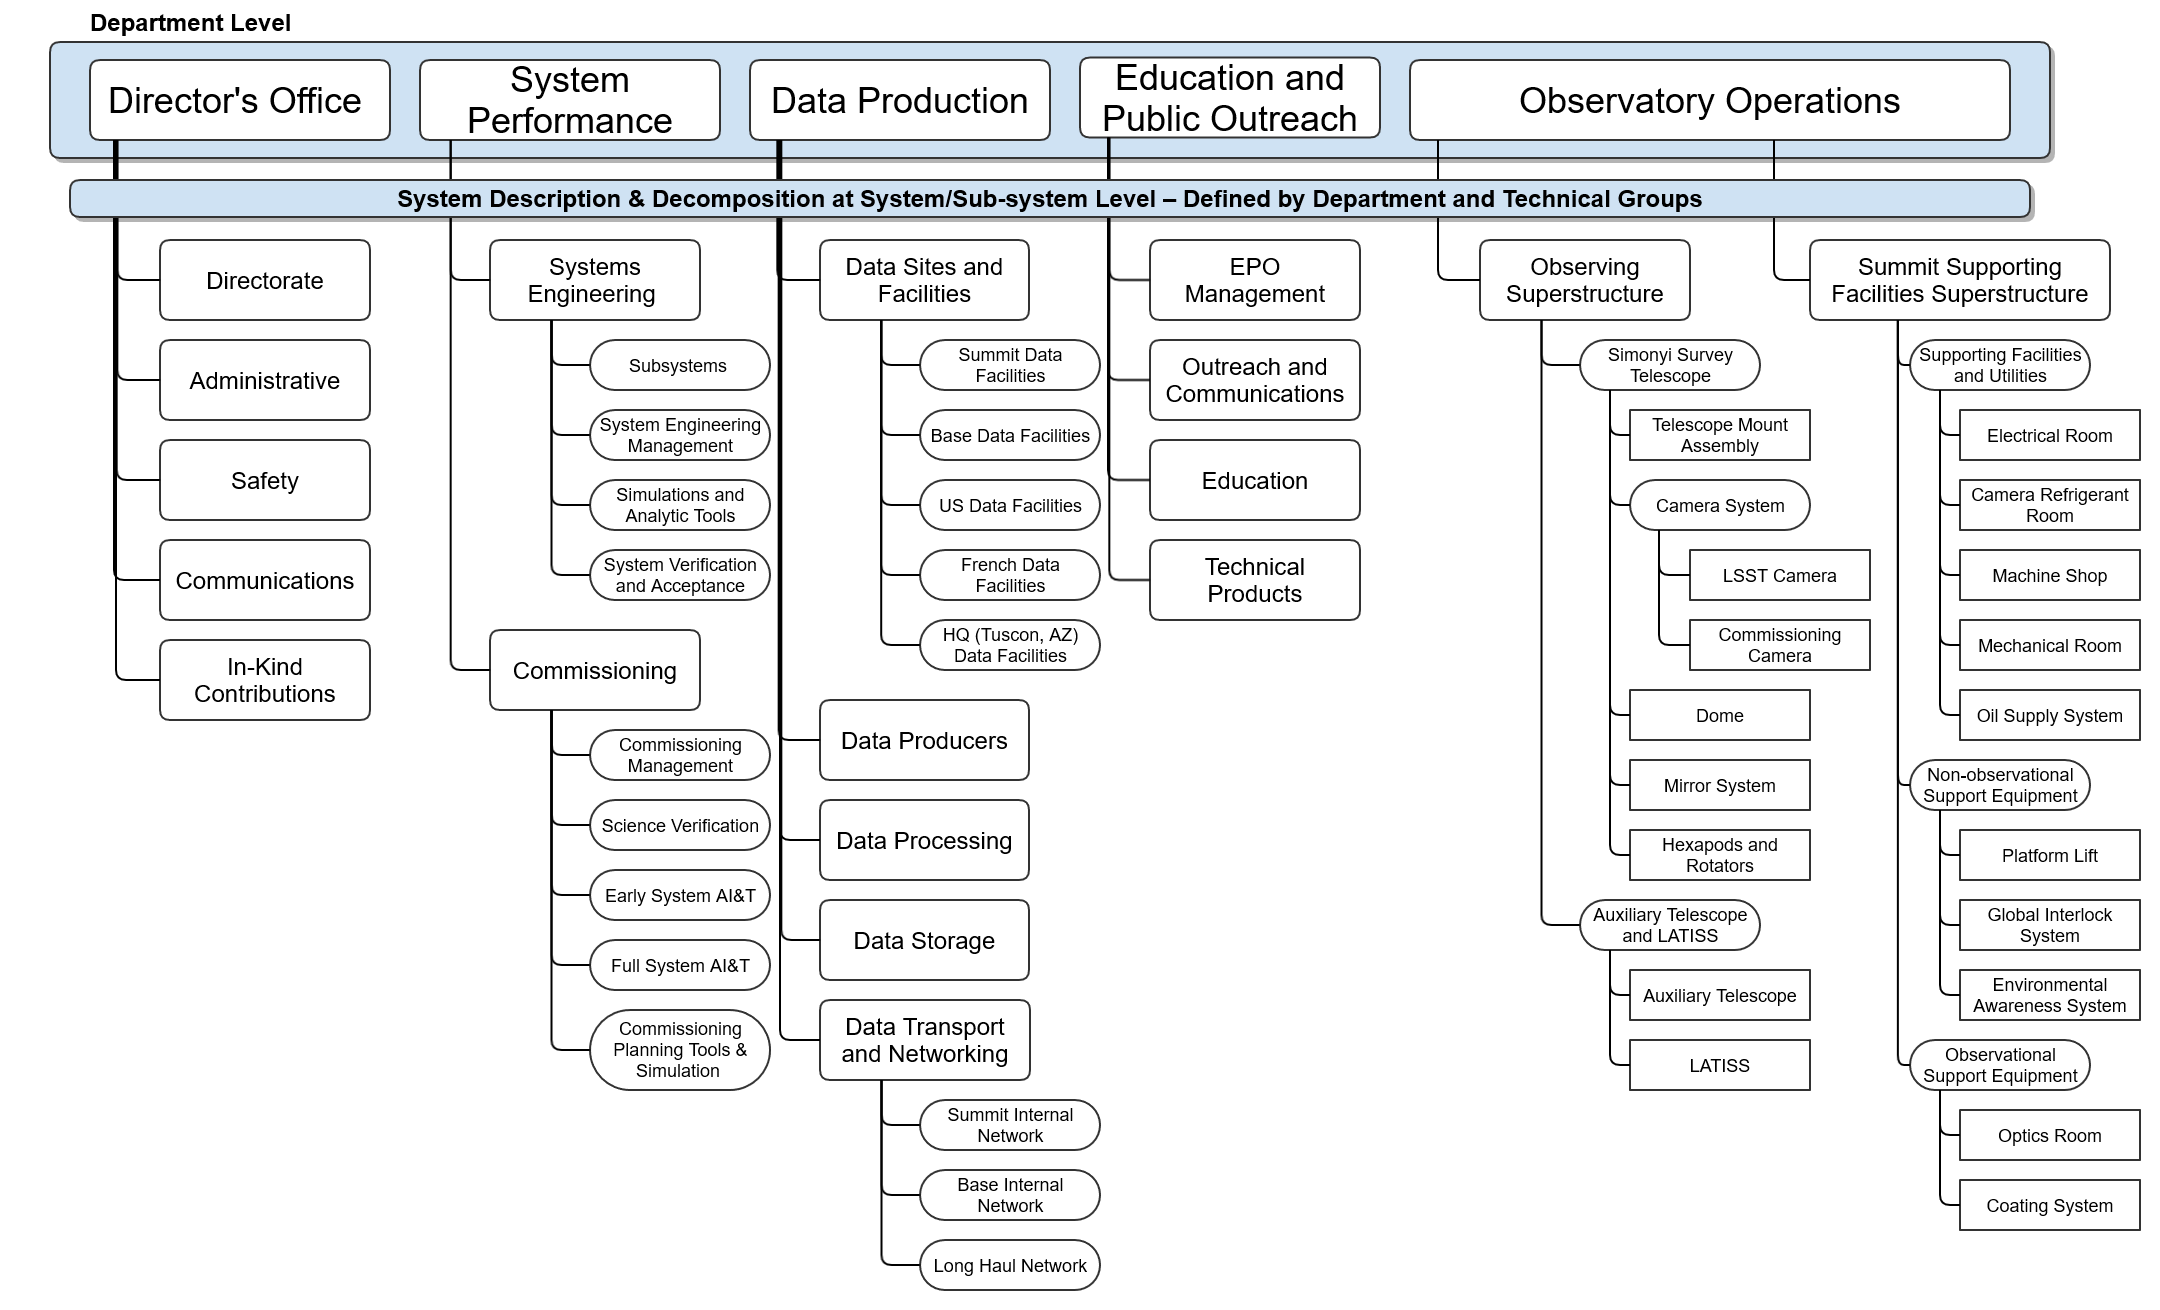
\includegraphics[width=\textwidth]{product-view-departments-decomposition-example}
\caption{Example of Department Decomposition at System and Subsystem Level.}
\label{fig:product-view-departments-example}
\end{figure}

Figure \ref{fig:product-view-auxtel-technical-design-example} is a more comprehensive example of AuxTel, depicting the Technical Design generic category.
Each category (yellow) and each subcategory (blue) from the Technical Design is addressed such that the reader has an idea of what the system is, how it is used, and documentation with references therein for retrieving critical information.
Note that physical interfaces are not address in the example.

\begin{figure}[htp!]
\centering
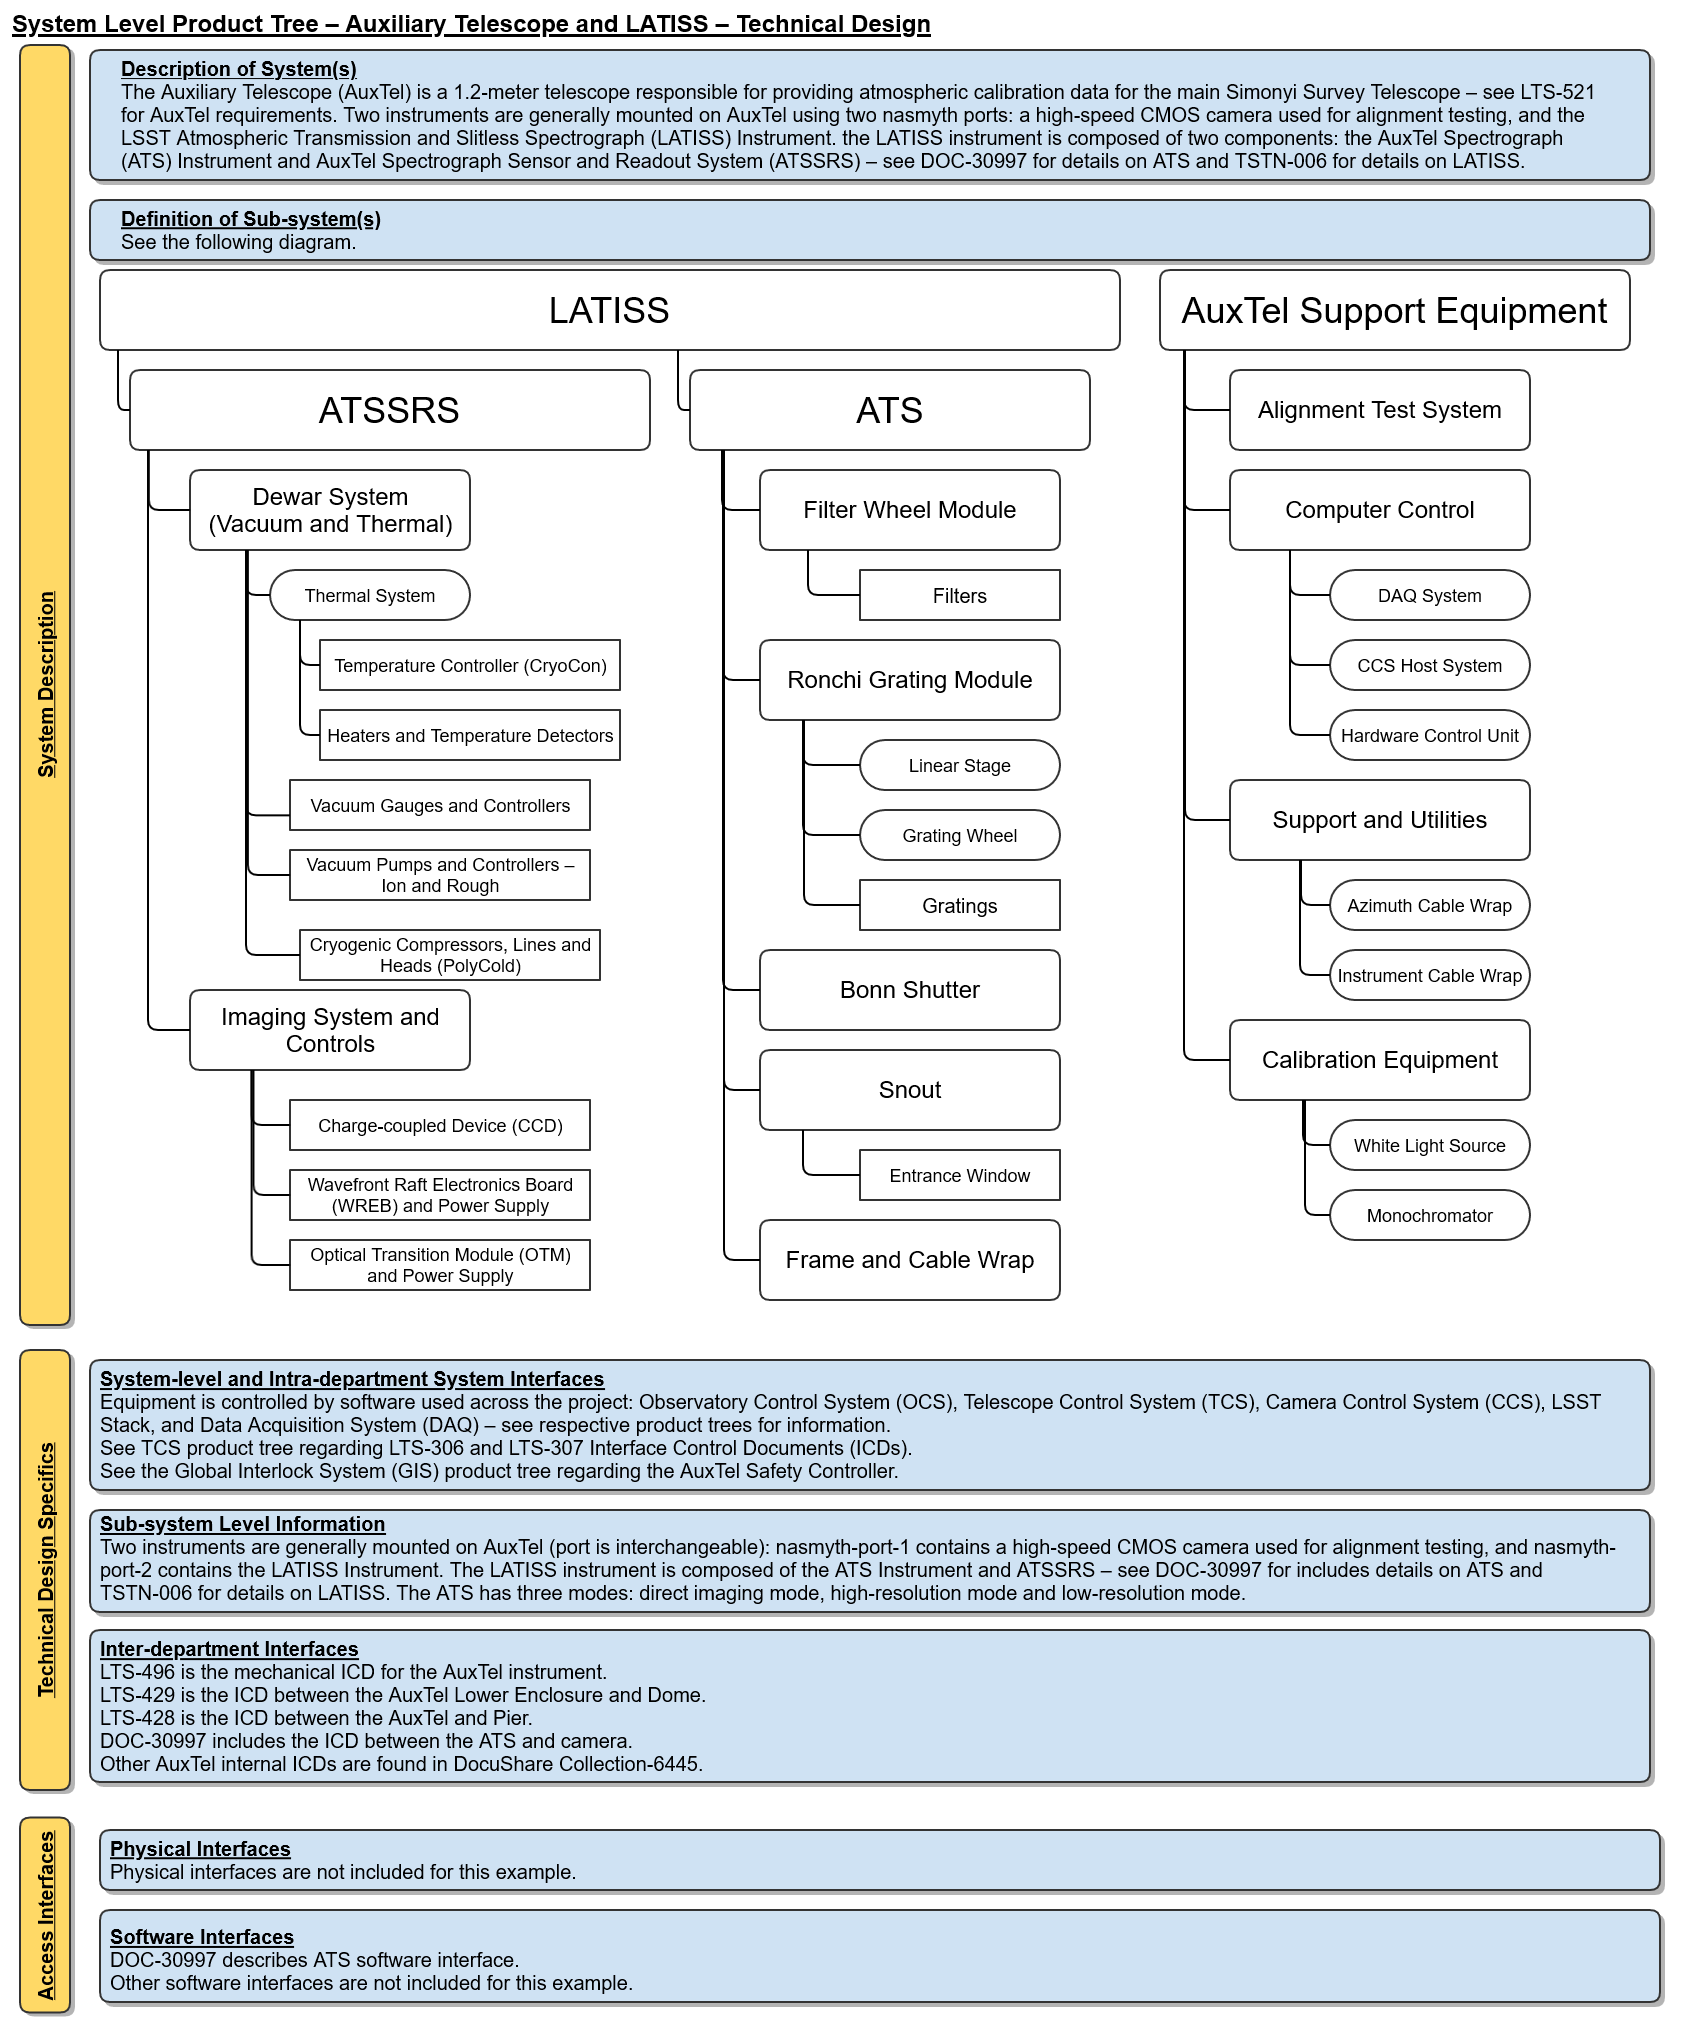
\includegraphics[width=\textwidth]{product-view-auxtel-product-tree-technical-design-example}
\caption{Example of Technical Design Generic Category from Product View, for an Auxiliary Telescope Subsystem.}
\label{fig:product-view-auxtel-technical-design-example}
\end{figure}

While it may seem Figure \ref{fig:product-view-departments-example} and Figure \ref{fig:product-view-auxtel-technical-design-example} are part of one example, that is not the case.
As previously described, it would be beneficial to organize the Product View to leverage the replicated information such as common software.
This was not considered for the two figures.

As another example of the Product View, Table \ref{table:product-view-department-ownership-example} shows how multiple departments can separate their responsibilities between a few high-level requirements and operational needs.
With well defined responsibilities, teams can communicate more effectively and the normative source of information should be identifiable.

\begin{table}[]
\begin{tabular}{|l|l|l|l|}
\hline
 & \textbf{\begin{tabular}[c]{@{}l@{}}Rubin Observatory\\ Operations\end{tabular}} & \textbf{\begin{tabular}[c]{@{}l@{}}System\\ Performance\end{tabular}} & \textbf{\begin{tabular}[c]{@{}l@{}}Data\\ Production\end{tabular}} \\ \hline
\textbf{\begin{tabular}[c]{@{}l@{}}Technical\\ Design\end{tabular}} & \begin{tabular}[c]{@{}l@{}}ICDs/IDDs\\ Requirements\end{tabular} & \begin{tabular}[c]{@{}l@{}}Validation of\\ Science Platform\end{tabular} & \begin{tabular}[c]{@{}l@{}}Science Platform\\ Design and Operations\end{tabular} \\ \hline
\textbf{Procedures} & \begin{tabular}[c]{@{}l@{}}Day/Night Shift Turn-over,\\ Energy Isolation Protocols,\\ Calibration Procedures\end{tabular} & \begin{tabular}[c]{@{}l@{}}Predictive Analysis,\\ Hazard Validation\end{tabular} & \begin{tabular}[c]{@{}l@{}}Data Release and\\ Prompt Alerts\\ Processing\end{tabular} \\ \hline
\textbf{Evaluation} & \begin{tabular}[c]{@{}l@{}}Verification Test Plans,\\ Failure Effects,\\ Test Reports\end{tabular} & \begin{tabular}[c]{@{}l@{}}Failure Mode and\\ Effect Analysis\end{tabular} & \begin{tabular}[c]{@{}l@{}}Assertion\\ Testing\end{tabular} \\ \hline
\end{tabular}
\label{table:product-view-department-ownership-example}
\end{table}

\subsection{Storage View}

Describe here the properties of the Storage View and provide diagrams showing the proposed structure for this view.
\subsection{Access View}
\label{sec:access-view}

The \emph{Access View} is a method of categorizing information into trees serving role-based needs to stakeholders.
It's purpose is to assist users in retrieving and discovering documentation and information applicable to their use cases.
As such, the access trees will be tailored to use case and role-based needs.
The Access View is be agnostic to the storage location because access is provided through the Documentation Portal so users do not need to know the repository for information.

The following subsections include four recommended trees for the Access View developed by the Documentation Working Group: Operational Access View, Safety Access View, Scientific Access View, and Engineering Access View.
It was natural to develop an Access View tree from a system decomposition, but it is useful for the project to determine if there are more efficient or natural trees, such as activity-based trees.
For each Access View tree, there are many ways and reasons to break the tree into the root-nodes.
With such sprawling associated subjects, it's more crucial to develop a strategy to break these root-nodes and leaf-nodes by considering categories, impacts to users, and how users would want to find associated information.

\subsubsection{Operational Access View}

The Operational Access View tree is intended to help with interfaces of real-time data and visualization, observations and its programming, and system state.
Figure \ref{fig:access-view-operational-example} is an example of the Operational Access View.
It may be natural to have separate leaf-nodes for the Main Telescope and AuxTel, capturing specific differences such as control interfaces.
Another natural break down could be day- and night-time operations, as shown in Figure \ref{fig:access-view-day-night-operations-example}.
Responsible groups should take advantage of commonalities and referential nature of the Documentation Views.
Users include use of equipment control devices, procedures and protocols for operation and maintenance, such as control room staff, viewing assistants.

\begin{figure}[ht]
\centering
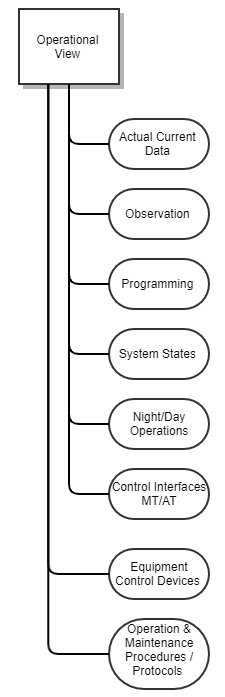
\includegraphics[scale=0.7]{access-view-operational-example}
\caption{Example of Operational Access View Tree with Root-nodes.}
\label{fig:access-view-operational-example}
\end{figure}

\begin{figure}[ht]
\centering
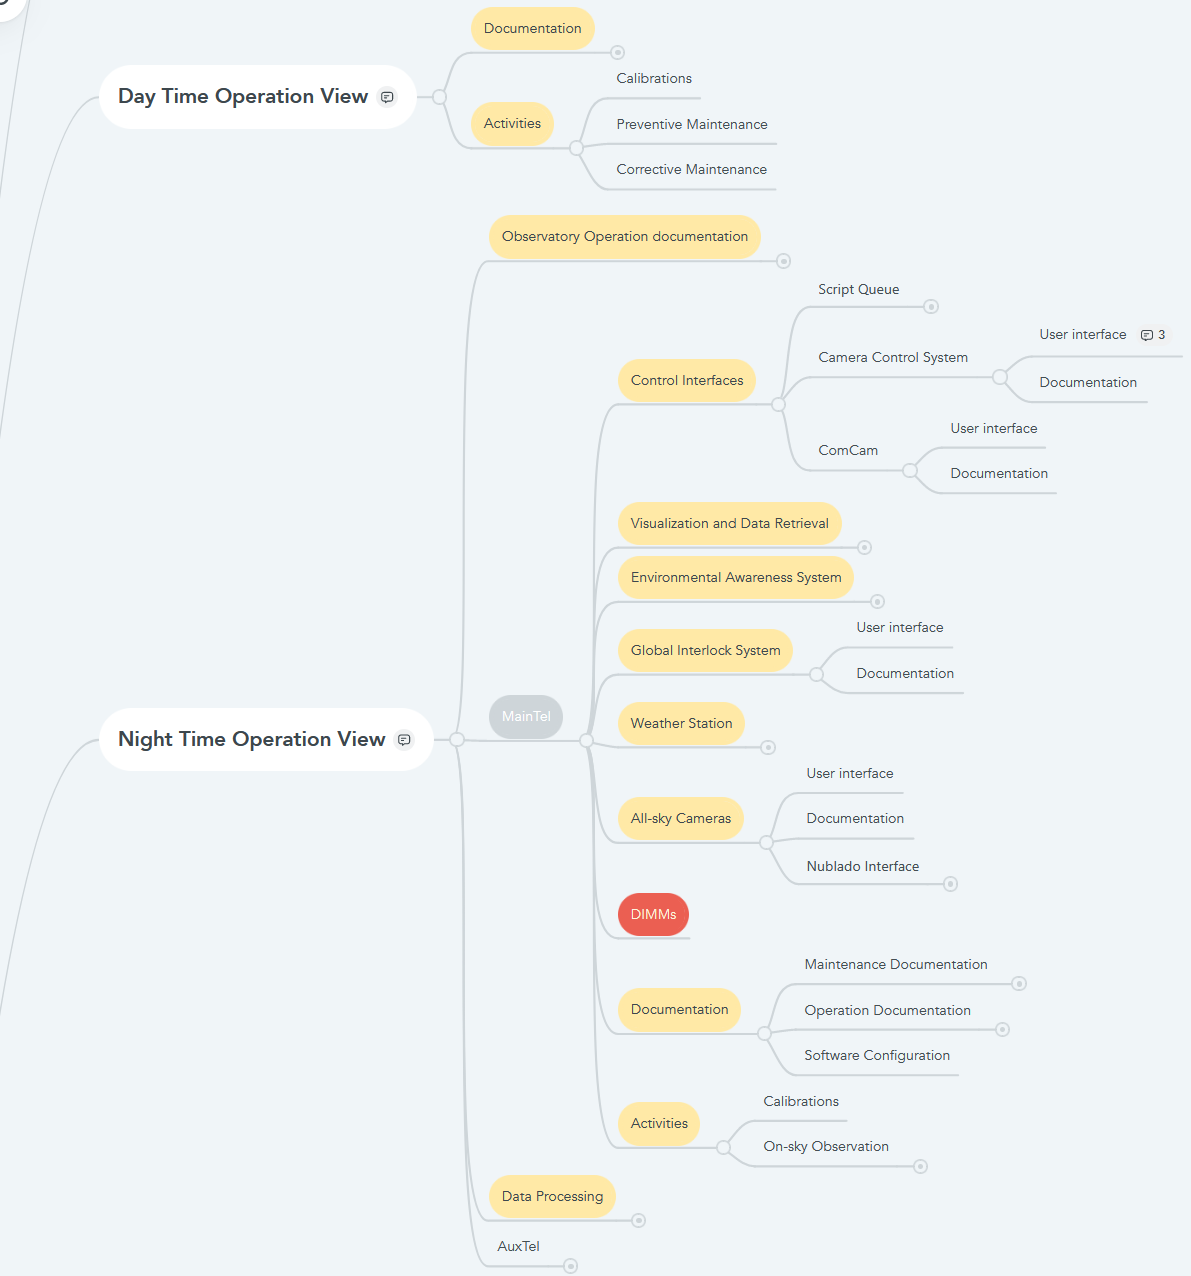
\includegraphics[width=\textwidth]{access-view-day-night-operations-example}
\caption{Example of Operational Access View Tree from Daytime and Nighttime Operations.}
\label{fig:access-view-day-night-operations-example}
\end{figure}

\subsubsection{Safety Access View}

The Safety Access View tree focuses on accessing information related directly to safety procedures and protocols that apply to the different systems.
This can help add consistency and verify requirements.
This tree would lead users to general safety procedures, specific safety procedures, emergency procedures of telescope and summit facilities (excludes emergency response).
The example provided by Figure \ref{fig:access-view-safety-example} includes safety and security aspects.
Users include safety, engineering, security, maintenance staffs and management.

\begin{figure}[ht]
\centering
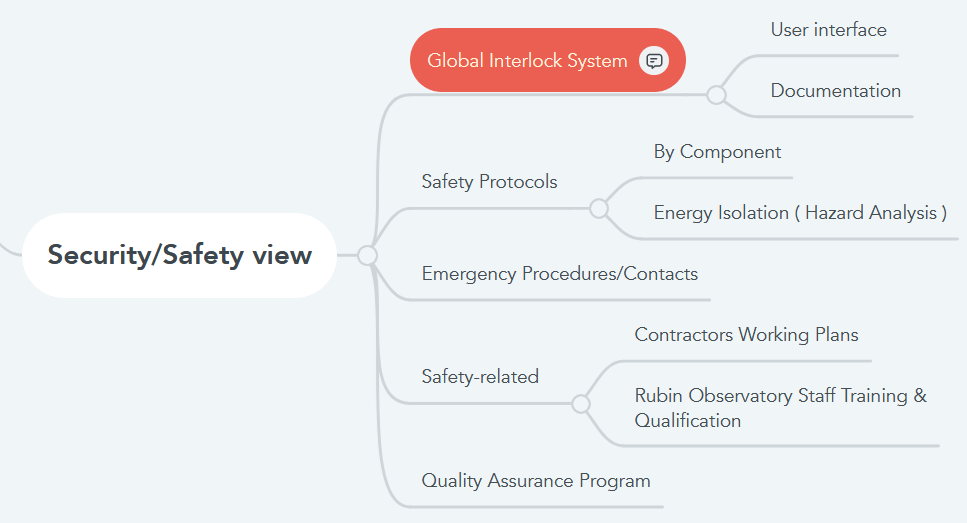
\includegraphics[width=\textwidth]{access-view-safety-example}
\caption{Example of Safety Access View Tree.}
\label{fig:access-view-safety-example}
\end{figure}

\subsubsection{Scientific Access View}

The Scientific Access View tree is for scientific platforms and interfaces that correspond or impact Rubin Observatory science objectives.
It is intended to ease access to the information by providing a clear list of the software and various databases.
An example is provided by Figure \ref{fig:access-view-scientific-example}.
Users include scientific, engineering, and observing staff and management.

\begin{figure}[ht]
\centering
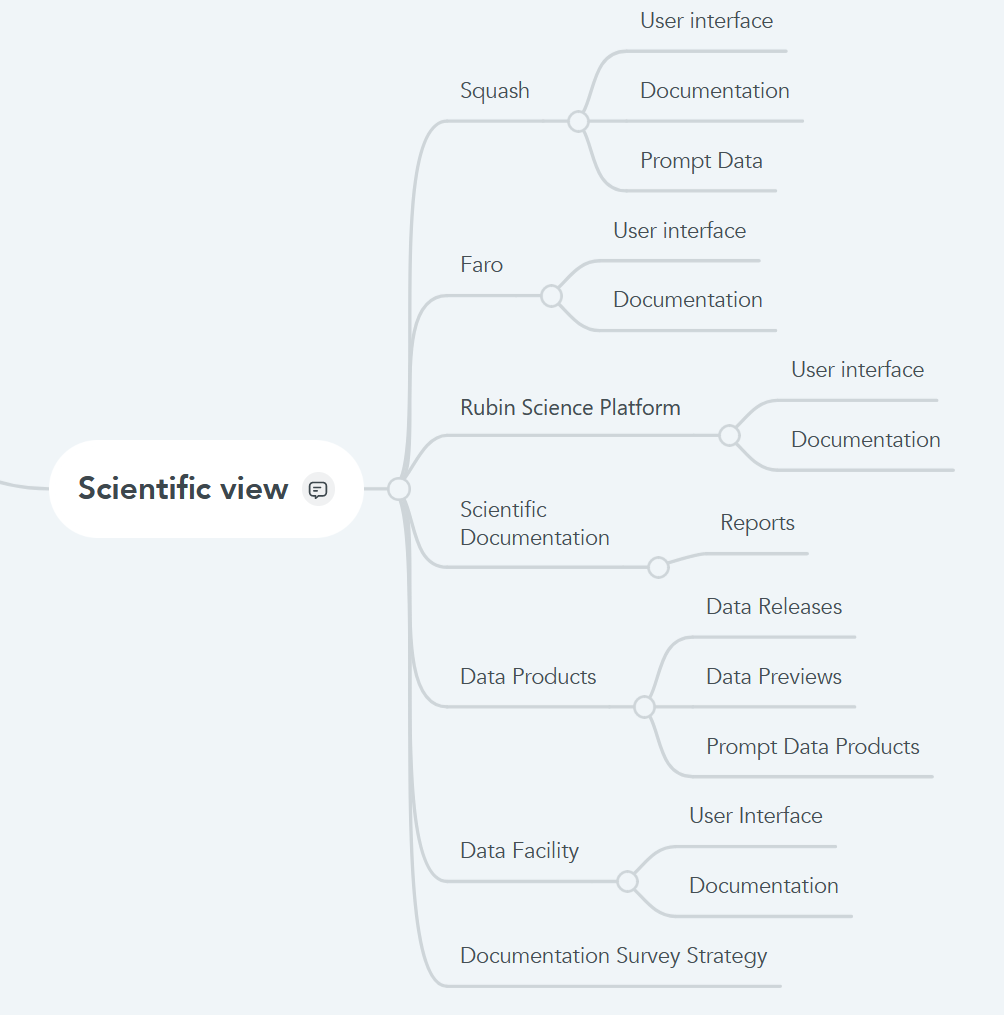
\includegraphics[width=\textwidth]{access-view-scientific-example}
\caption{Example of Scientific Access View Tree.}
\label{fig:access-view-scientific-example}
\end{figure}

\subsubsection{Engineering Access View}

The Engineering Access View tree is for accessing Rubin Observatory technical information.
In addition to the technical documentation, access interfaces and facility-related data would be needed.
An example is provided by Figure \ref{fig:access-view-engineering-example}.
Users include staff and management involved in system performance and system engineering activities.

\begin{figure}[ht]
\centering
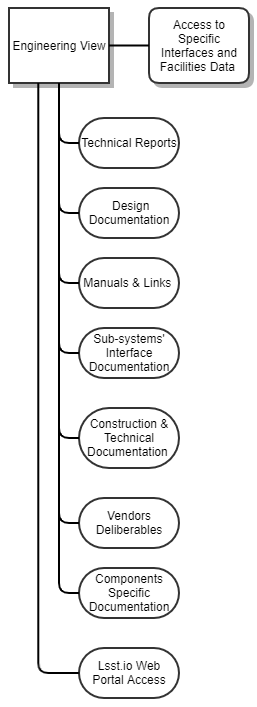
\includegraphics[scale=0.7]{access-view-engineering-example}
\caption{Example of Engineering Access View Tree.}
\label{fig:access-view-engineering-example}
\end{figure}

\subsection{Topic View}

The \emph{Topic View} aimes to categorize information into domain specific document types.
Its purpose is to allow users the ability to find information of a specific form within a documentation system (\it{e.g.} 3D CAD models).
It first requires a defined decomposition of systems, subsystems and components.
% The sentance above seems to be at odds with the narrative in the "Product View" sectiom
Topics could range to any categorization, such as physical location or department ownership.
The Topic View must be agnostic to the storage location because it requires an access portal to utilize it, such as the Rubin Documentation Portal (Section \ref{sec:DocPortal}).
The construction of a Topic View tree depends on the implementation of the portal, the purpose of the topic tree, and the targeted user base.

The Documentation Working Group suggests the following categories to define a system for the Topic View:

\begin{itemize}
\item design documents
\item requirement documents
\item technical manuals (e.g., operation or maintenance)
\item operational documents (e.g., procedures)
\item data performance
\item evaluation processes
\item maintenance reports
\item safety and hazard mitigations
\item access and software
\end{itemize}




\subsection{The Documentation Portal}
\label{sec:DocPortal}

The working group recommends the creation of a \emph{documentation portal} web application as a means of making documentation content discoverable and accessible to Rubin Observatory staff.
The documentation portal provides interfaces for both searching (based on content and metadata) and browsing (based on hierarchical categorization) of documentation resources. Documentation does not reside within the portal itself.
Rather, the portal's objective is to efficiently link the user to the document where it is stored in any of the observatory's adopted storage platforms (Section \ref{sec:primary-sources}).
The portal discussed here is based upon the www.lsst.io website, which provides a search and browsing interface for the Rubin Observatory's public-facing technical documentation.
The new portal will be accessible only those with Rubin Observatory staff credentials, and will be purpose-built for observatory and survey operations.
This section describes the design principles, technical architecture, security model, and cost estimate of the Rubin Observatory documentation portal.

\subsubsection{Design requirements}

The design requirements of the documentation portal reflect the recommendations made by the Documentation Working Group elsewhere in this report:

\begin{enumerate}
  \item The role of the documentation portal is to link to documentation resources. The portal itself does not host the content itself, or provide user interfaces for creating and maintaining new versions of documentation content. This requirement reflects the working group's recommendation that documentation content should be hosted on a select set of platforms that are idiomatic for the content and the teams that work with that content (Section \ref{sec:primary-sources}).

  \item The documentation portal must provide equal support for content stored in any of the working group's recommended storage platforms.

  \item The documentation portal must be capable of supporting several hierarchical browsing schemes for accessing content based on different organizational views of the documentation (Section \ref{sec:views}).

  \item The documentation portal should automatically update and sort documentation content, to the greatest extent possible. In other words, curators should only need to maintain documentation in the document's storage platform, without any administrative action through the documentation portal's UI. A consequence of this requirement is that the documentation portal should not persist information about a document that is not available from the document's own storage platform.

  \item The documentation portal should be secured so that it is only accessible to users with Rubin Observatory staff credentials.

  \item The documentation portal should not maintain fine-grained access control for specific documents or categories of documents. For secured documents, the portal relies upon the security mechanisms of the document's own storage platform. The portal should also reduce its metadata storage of confidential documents to ensure that content cannot be inferred from a search, for example.
\end{enumerate}

\subsubsection{Technical architecture}

The architecture described here is based upon that which is already put into production with the www.lsst.io portal for public-facing documentation. Starting from this working archetype relieves a great deal of technical risk and development from the new portal's implementation. Both portals share the use of Algolia as a search backend and Ook as a content indexing service. The documentation portal discussed here will have an independent front-end to support the specific access views recommended by the working group. The documentation portal will also use a separate instance of the Algolia database to eliminate any risks associated with leaking internal documentation to the public-facing www.lsst.io portal.

Figure \ref{fig:portal-arch} depicts the components of the documentation portal.

\begin{figure}[t]
\caption{Architecture of the documentation portal. Users find documents on the portal application, which in turn provides links into the original documentation repositories. Data in the portal application is supplied by the Algolia search service, which in turn gets its metadata from the original documents in their repositories via the Ook indexing service.}
\centering
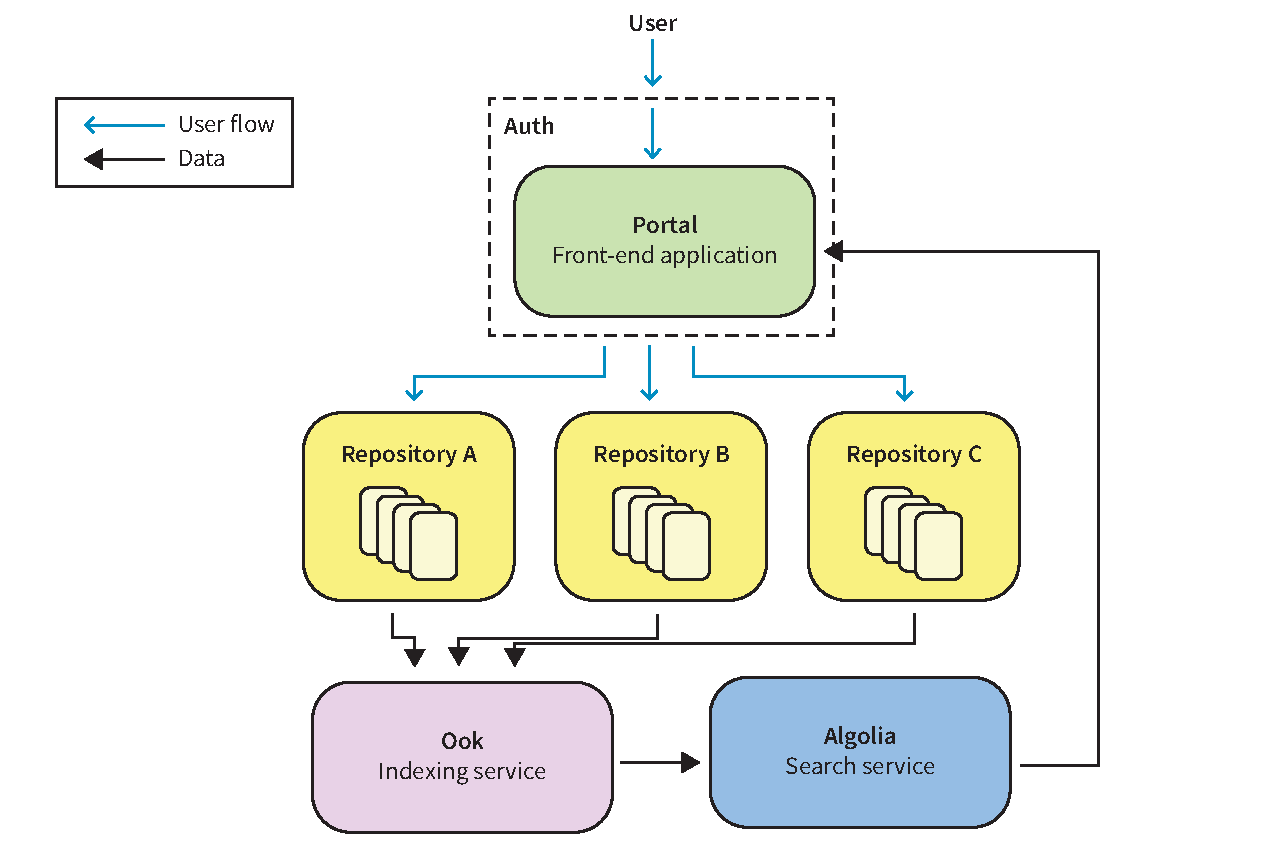
\includegraphics[width=\textwidth]{portal-architecture}
\label{fig:portal-arch}
\end{figure}

\paragraph{Algolia}

The core function of the portal is to enable access to documentation through browsing and search. To implement this, the portal needs a back-end service that contains metadata about Rubin's documentation holdings and provides interfaces to access and query that metadata from the front-end (website). This search database and interface could be made for "free" with entirely open-source components such as Elasticsearch and in-house web service. However, a search database and service are sufficiently generic that we cannot add value by making it in-house, and in fact developing, tuning, and operating this service, would costly in terms of labor. For the www.lsst.io public documentation portal, we opted to use Algolia and recommend that we make the same choice for the observatory's documentation portal.

Although www.lsst.io is currently operating on a free open-source license of Algolia, the observatory's internal documentation portal would be an entirely paid license. Algolia prices based on record counts and request rates. In operating www.lsst.io, we found record count to be the limiting factor. At the moment, 1000 records costs \$1 per month. 1,000,000 records would cost \$850 per month with volume discounts. For reference, the www.lsst.io service currently uses 110,000 records to host all technical notes and change-controlled documents with drafts hosted on lsst.io.

Note that a single document is composed of potentially many records in Algolia. To optimize full-text search, we break a document into smaller records, generally across section boundaries. Our current algorithms generally produce small record, so it is possible to reduce costs by tuning how we segment content into Algolia records. Furthermore, each sorting option requires a separate pre-sort index. Sorting documents by date, and document number, in addition to relevance, consumes three times as many records as only sorting by relevance.

\paragraph{Ook}

The Ook service is responsible for continuously indexing content into Algolia. Whereas we chose Algolia to provide a turn-key search database service, for www.lsst.io we chose to build the indexing service in-house to have complete control over how documents are indexed, and what metadata is associated with each document. For example, LaTeX-based documents are indexed based on metadata exported from the Lander PDF landing page generator (also developed in-house), which in turn parses LaTeX syntax in the document source to access metadata such as titles, authors, and so on. The configurability of Ook is beneficial to indexing other types of highly specialized documentation.

The key design principle of Ook is that metadata is extracted from the document as it appears in its repository, rather than requiring direct human interaction with Ook or Algolia to curate the data. This allows Ook to scale well across an organization as large and varied as Rubin because individual teams manage documents as they already do in the repositories they are already familiar with.

Ook is built such that new content types can be added by writing additional Python-based workflows for each content type. Ook itself provides utilities for queuing ingests, converting content and formatting data for Algolia, and working with the Algolia service itself.

Ook indexing operations can be triggered several different ways. For example, the lsst.io service publishes messages to a Kafka cluster whenever documentation is published on that platform; Ook subscribes to those messages and queues indexing workflows. Ook indexing operations can also be scheduled through an HTTP API. Generally, the goal is to trigger indexing operations automatically whenever the source material changes.

The existing Ook indexing workflows work by downloading content from websites and web services (HTTP APIs). If content is not easily accessible, it would be possible to develop an alternative workflow, such as submitting copies of the document directly to Ook for indexing. Some document repositories may offer online access but have hard-to-use APIs (such as DocuShare). These difficulties can be worked around, for example by emulating a web browser to download content and metadata, but at the cost of more fragile indexing workflows.

Ook is currently operated as a Kubernetes application in the Google Cloud. This arrangement is ideal for minimizing operations cost, and providing convenient scaling.

\paragraph{Front-end application}

The front-end web application is how users (Rubin Observatory staff) find documentation. The web application does not provide the document itself—instead, the web application provides a search result card that the user can click on to access the document in its original repository. The Algolia services provides all browsing and search functionality; the front-end application provides the user interface over top of Algolia.

In addition to providing a link to the original document, the portal can also provide an immediate view of a document's metadata. Although the front-end application can show a basic view of a document's metadata based on metadata common to all records, the website can be developed to show additional metadata for different types of documents.

For www.lsst.io, we built the site as a React JavaScript application. This allowed us to use and customize the pre-made widgets provided by Algolia for building the user interface.

The front-end application will be accessible only to users who log in. The simplest way to approach this is by putting the application behind a VPN so that the application is completely separate from security concerns. Another approach would be to place the application behind an OAuth proxy to provide a slightly better user experience.

\subsubsection{Support for multiple views}

In Section \ref{sec:views}, the documentation working group outlines several views for hierarchically arranging documents trees. These views correspond to navigational structures in the front-end application. Although the front-end application code is generally "aware" of the different trees, individual documents are placed in the tree on the basis of metadata in their Algolia records, so that the Algolia service can pre-sort and filter documents into the trees. Since Ook supplies metadata to Algolia, and Ook in turn leverages metadata native to the document and the document's repository, the responsibility for curating documents into different views is the responsibility of individuals managing documents in each repository.

\subsubsection{Information security}

Documentation has multiple types of security concerns, such as control over who and how documents are updated, control over who can access documents, and ensuring the long term integrity and preservation of information. Since the documentation portal is not the canonical repository for any documentation, the portal is not involved in controlling document updates and preservation. The portal's key security concern is access control.

The portal is designed to only provide authentication-based access control. Any Rubin staff member with credentials can access any metadata records contained within the documentation portal. Once a user selects a document to view, they are forwarded to that documentation repository and must authenticate with that repository and be subject to its access control rules.

However, the metadata contained in the documentation portal can be potentially rich, even including the full-text content of a document to enable search functionality. It is conceivable that some of this metadata may not be appropriate for observatory-wide access (such as information with export controls, for example). In these cases, the most realistic approach to preserving strict access controls in these situations is to limit what metadata is available. In order of strictness, the following approaches can be used:

\begin{enumerate}
  \item Omit full-text content of a document from Algolia records.
  \item Limit or obfuscate other metadata (such as titles) in the Algolia records.
  \item Omit the individual documents altogether from Algolia and instead link to a documentation landing page hosted by the secure document repository itself.
\end{enumerate}

In all cases, controlling how documents are indexed is done by configuring the indexing service, Ook.

\subsubsection{Effort estimate}

The key tasks for implementing this plan are:

\begin{enumerate}
  \item Building additional content indexing workflows into Ook and updating the metadata schema to accommodate all use cases.
  \item Build the documentation portal application.
  \item Curate documents so that they are uniformly present in their document repositories and have any metadata that is expected by the Ook indexing workflows.
\end{enumerate}

The last task category can be distributed to teams working in each document repository.

To provide a sense of the scale of the first two tasks, the implementation of the www.lsst.io portal is a useful reference. Building the first version of Ook, which indexes LaTeX documents and Sphinx-based technical notes in lsst.io required 4 weeks of work. Building the front-end website required 6 weeks.

Since that original implementation, we have gained more experience building React web applications and working with Algolia, so we can expect less than 4 weeks of work to build out the internal web application. Although Ook can be expanded as is, the key uncertainly is in the number and complexity of the additional indexing pipelines that need to be built for additional document types and repositories. Generally, though, an internal documentation portal can likely be stood up within 1 to 3 months, with a potential long tail of effort to continue to add support for additional content types.


\section{Lingual translations}

Due to the nature of the Rubin Observatory, it is inevitable that some documents will need to be translated into other languages.
The major need will be English and Spanish translations for the American and Chilean operational locations.
It is a significant yet inevitable undertaking for bilingual translations throughout the observatory lifetime.
English/Spanish bilingual documents will be needed, and they must be available with up-to-date information to prevent issues during construction and maintenance.
The accuracy of language is crucial (e.g., context, terminology), from work instructions to inclusivity (e.g., engagement in continuous improvement).
The risk of improper or unavailable translations can generally impact the schedule (e.g., delay in work) and results increased risk to personnel, equipment, the environment or security when procedures or protocols cannot be accurately followed.

The Documentation Working Group recommends that, at a minimum, the following translated in both, English and Spanish:
\begin{itemize}
	\item procedure documents and manuals for activities conducted on a routine basis,
	\item any and all safety documents, and
	\item websites that facilitate the organization and location of translated documentation (e.g. DocuShare).
\end{itemize}
Any other documents, drawings, schematics, parts lists, etc. should be translated on an as-needed basis.

Workflows for documentation should include steps to determine if translation is needed and its implement, as defined by the project of technical group.
The determination and reason for translation should be recorded; i.e., required, preferred, suggested or unneeded.
When releasing documents, at least one approver should be designated specifically to confirm that the translated version matches the original.
This is especially important when revisions are made, to ensure any changes are fully and accurately captured.
It should be clear within the document or applicable sections which have translation and the respective location(s).

When producing translations, the Documentation Working Group recommends that they are reviewed by a technically-competent bilingual person.
For version-controlled documents, it is recommended that original and translated versions be kept in a single file.
The location for translated documents can be done in whatever format is most appropriate for the document; e.g., a schematic might have both English and Spanish labels next to each other, or a procedure may be written entirely in English and then repeated in Spanish.

The construction project should be involved as much as practical, but the effort will continue into operations.
Additionally, the Documentation Working Group believes it is a requirement for the project to allocate resources for ongoing support throughout operations.
While estimating the resources needed for this, it is recommended to consider additional translation needs for global associations, including user-facing scientific documentation.


\newpage
% Include all the relevant bib files.
% https://lsst-texmf.lsst.io/lsstdoc.html#bibliographies
\section{References} \label{sec:bib}
\renewcommand{\refname}{} % Suppress default Bibliography section
\bibliography{local,lsst,lsst-dm,refs_ads,refs,books}

% Make sure lsst-texmf/bin/generateAcronyms.py is in your path
\section{Acronyms} \label{sec:acronyms}
\addtocounter{table}{-1}
\begin{longtable}{p{0.145\textwidth}p{0.8\textwidth}}\hline
\textbf{Acronym} & \textbf{Description}  \\\hline

API & Application Programming Interface \\\hline
HTTP & HyperText Transfer Protocol \\\hline
IT & Information Technology \\\hline
LSE & LSST Systems Engineering (Document Handle) \\\hline
LaTeX & (Leslie) Lamport TeX (document markup language and document preparation system) \\\hline
PDF & Portable Document Format \\\hline
SE & System Engineering \\\hline
UI & User Interface \\\hline
VPN & virtual private network \\\hline
\end{longtable}

% If you want glossary uncomment below -- comment out the two lines above
%\printglossaries

\end{document}
